\section{Pre-Training}

\subsection{Pre-Training Data}                        
\kimi{3} is pre-trained on a curated corpus spanning four primary text
domains---Web Text, Code, Mathematics, and Knowledge---together with a
large-scale vision corpus. The vision data covers captions, interleaved image--text
documents, OCR, perception, video, and visual coding data. Our
data pipelines build on those developed for \kimi{2}~\citep{kimiteam2025kimik2openagentic} and
refined in \kimi{2.5}~\citep{kimik25}.                                                                                                            
 \paragraph{Text data} Each domain is filtered by a combination of rule-based heuristics, classifier-based quality scoring, and deduplication, with domain-specific sampling rates determined by ablation studies on smaller models. Following the rephrasing recipe of \kimi{2}~\citep{kimiteam2025kimik2openagentic}, we rephrase knowledge and mathematics corpora with style and perspective-diverse prompting, chunk-wise autoregressive generation, and fidelity verification against the source documents.                   

 
 \paragraph{Vision data} The vision corpus follows the taxonomy of \kimi{2.5}~\citep{kimik25}, combining open-source collections with in-house pipelines for filtering, synthesis, and deduplication.
 During training, coordinate supervision is provided in both absolute and normalized ([0,1]) formats, enabling precise and resolution-robust localization.
 In addition to classical text-captioned images, we substantially scale up programmatic multimodal data, coupling code snippets with their rendered visuals across domain-specific formats including SVG, 3D assets, Webpage, Game, and CAD schematics.


\subsection{Scaling Law}
\begin{figure}[t]
    \centering
    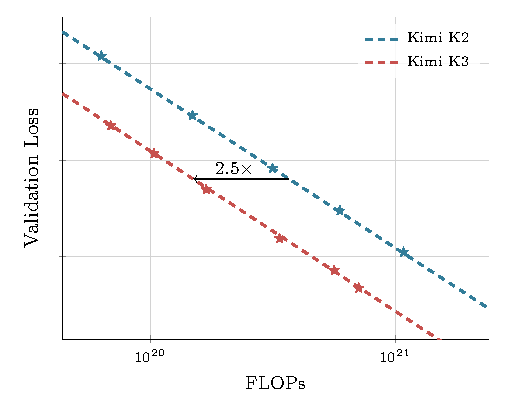
\includegraphics[width=0.55\linewidth]{figures/scaling-law.pdf}
    \caption{
        Fitted scaling-law curves for \kimi{2} and \kimi{3}.
        \kimi{3} achieves ~$2.5\times$ gain in scaling efficiency over \kimi{2}.
    }
    \label{fig:scaling-law}
\end{figure}
Taken together, the architectural, data, and training improvements described in the previous sections define our new model family. Since these changes also alter the optimal training regime, we conduct dedicated scaling-law studies to retune key hyperparameters, including the batch size, learning rate, tokens-per-parameter ratio (TPP) and the model shape. Evaluated on held-out OOD validation data, the scaling law curves in (Fig.~\ref{fig:scaling-law}) show that these improvements collectively deliver an approximately $2.5\times$ gain in overall scaling efficiency over \kimi{2}. Table~\ref{tab:k2-k3-comparison} provides a detailed architectural comparison between \kimi{2} and \kimi{3}, highlighting the structural changes that contribute to this improvement.

Our scaling-law study consistently favors cosine decay over Warmup Stable Decay (WSD) \citep{hu2024minicpm}, leading us to adopt cosine decay as the default learning rate schedule. We compare cosine decay and WSD under a fixed minimum learning rate. Although prior work has reported that WSD can match or even outperform cosine decay, we observe that the two schedules exhibit markedly different optimal hyperparameters. Even under the same model size and training-token budget, their optimal peak learning rates and batch sizes differ substantially. As a result, comparing the two schedules using a shared set of hyperparameters may unfairly favor one simply because those hyperparameters are better aligned with it. To ensure a fair comparison, we conduct an independent scaling-law search for each schedule. Under their respective optimal hyperparameter settings, cosine decay consistently achieves a lower final loss than WSD.

\begin{table}[t]
    \centering
    \caption{Architectural comparison between \kimi{2} and \kimi{3}.}
    \label{tab:k2-k3-comparison}
    \small
    \renewcommand{\arraystretch}{1.08}
    \setlength{\tabcolsep}{7pt}

    \begin{tabularx}{0.94\linewidth}{
        >{\raggedright\arraybackslash}X
        >{\centering\arraybackslash}p{0.16\linewidth}
        >{\centering\arraybackslash}p{0.22\linewidth}
        >{\centering\arraybackslash}p{0.10\linewidth}
    }
        \toprule
        & \textbf{\kimi{2}}
        & \textbf{\kimi{3}}
        & $\boldsymbol{\Delta}$ \\
        \midrule
        Architecture
            & MoE
            & MoE
            & -- \\
        $\#$Layers
            & 61
            & 93
            & $\uparrow 52\%$ \\
        Total Parameters
            & 1.04T
            & 2.78T
            & $\uparrow 167\%$ \\
        Activated Parameters
            & 32.6B
            & 104.2B
            & $\uparrow 220\%$ \\
        Hidden Dimension
            & 7,168
            & 7,168
            & $=$ \\
        Latent MoE Dimension
            & --
            & 3584 (0.5×)
            & -- \\
        MoE Hidden Dimension per Expert
            & 2,048
            & 3,072
            & $\uparrow 50\%$ \\
        Routed Experts
            & 384
            & 896
            & $\uparrow 133\%$ \\
        Experts Active per Token
            & 8
            & 16
            & $\uparrow 100\%$ \\
        Shared Experts
            & 1
            & 2
            & $\uparrow 100\%$ \\
        Attention Heads
            & 64
            & 96
            & $\uparrow 50\%$ \\
        Number of Dense Layers
            & 1
            & 1
            & $=$ \\
        Vocabulary Size
            & 160K
            & 160K
            & $=$ \\
        Training Context Length
            & 128K
            & 1M
            & $8\times$ \\
        Attention Mechanism
            & MLA
            & Hybrid KDA--MLA
            & -- \\
        Activation Function
            & SwiGLU
            & SiTU-GLU
            & -- \\
        Attention-Layer Composition
            & 61 MLA
            & 69 KDA + 24 MLA
            & -- \\
        Number of MTP Layers
            & 1 layer
            & 1 layer
            & $=$ \\
        Total Parameters of ViT 
            & - 
            & 401M
            & - \\
        $\#$ViT Layers
            & - 
            & 27 layers 
            & - \\
        Patch Size of ViT
            & - 
            & 14
            & - \\
        $\#$Attention Heads of ViT
            & - 
            & 12 
            & - \\
        \bottomrule
    \end{tabularx}
\end{table}

\subsection{Training Recipe}



\kimi{3} adopts a native multimodal training strategy in which language and vision are jointly optimized from the start of training, rather than grafting a vision encoder onto a pre-trained language model through a post-hoc alignment stage. Under this paradigm, visual and textual tokens are interleaved within a single next-token prediction objective, enabling the shared backbone to learn unified multimodal representations from the outset.

We optimize the model using the Per-Head Muon optimizer (\S~\ref{sec:perhead_muon}) together with the weight-clipping mechanism introduced in \kimi{2}, while adopting QB (\S~\ref{sec:qb}) for MoE load balancing. We use a cosine learning rate schedule with a $1\%$ linear warmup. Weight decay is set to $0.1$ throughout.

Our pre-training begins with a context length of $8\mathrm{k}$ tokens, which is later extended to $64\mathrm{k}$ tokens in a subsequent training phase.






\subsection{Long-Context Extension}


\paragraph{Positional encoding}
\kimi{3} uses no explicit positional embedding (NoPE), and instead encodes positional information implicitly through the recurrent gating and decay mechanism of KDA.
As a result, the model extrapolates directly to 1M-token contexts without any positional-encoding modification, such as RoPE rescaling or interpolation~\citep{peng2023yarn}.

\paragraph{Long-context data}
Long documents and videos from natural sources contain a substantial amount of low-quality content, including near-duplicates, binary blobs, truncated files, video clips, and invalid machine-generated logs.
We therefore process them through a dedicated cleaning pipeline that combines exact and fuzzy deduplication, supplemented by perceptual hashing over frames for video, together with heuristic and classifier-based quality filtering, and structural validation.
Because genuinely long and coherent documents and videos are scarce relative to short text, we upsample them so that the long-context distribution is not overwhelmed by short sequences during cooldown. 
Length alone, however, does not confer long-range capability.
To address this, we synthesize additional long-context data by carefully permuting and concatenating multimodal documents and sub-tasks, so that the embedded tasks can be solved only by attending to information scattered across the full 1M-token context.
This trains the attention mechanism at the intended scale and prevents it from degenerating into local patterns.


\paragraph{Progressive context extension}
\kimi{3} supports a context window of up to 1 million tokens.
We achieve this through extending the context window progressively as training proceeds, following a four-stage curriculum.
The window grows from 8K to 64K tokens during pre-training, and from 256K to 1M tokens during the cooldown phase.
Concentrating the costly long-sequence computation within a small fraction of the overall training budget keeps the curriculum economical while still allowing the model to adapt gradually to increasingly long-range dependencies.
The sequence-dimension partitioning that makes million-token training tractable for the KDA layers is described in \S\ref{sec:kda-cp}.




